% Common header => These packages are almost always used, so why not always import them and not think about it
\documentclass[]{article}
\usepackage[T1]{fontenc}
\usepackage[utf8]{inputenc}
\usepackage{graphicx}
\usepackage{siunitx}
\usepackage{booktabs}
\usepackage[table]{xcolor}
\usepackage{soul}
\usepackage[longnamesfirst,sort]{natbib}
\bibpunct[, ]{(}{)}{;}{a}{,}{,}% Citation support using natbib.sty
\renewcommand\bibfont{\fontsize{10}{12}\selectfont}
\usepackage{amsmath}
\usepackage{amsfonts}
\usepackage[hidelinks]{hyperref}
\usepackage[all]{nowidow}
\newcommand{\rref}[2][\!\!]{\hyperref[#2]{#1~\ref{#2}}}
\usepackage{textcomp}
\usepackage{gensymb}
\usepackage{lmodern}

% Uncomment the following for special packages
% \usepackage[printwatermark]{xwatermark}
% \newwatermark[allpages,angle=45,scale=3,xpos=0,ypos=0]{DRAFT}
\usepackage[french]{babel}

% Revision tools => These commands (\comment, \commentbox, \addref and \xx) are used for revising a document and leave some comments
\usepackage{xspace} 
\newcommand\comment[2]{\hl{#1}\xspace}
\newcommand\commentbox[1]{
\vspace{12pt}

\fbox{\begin{minipage}[c]{.90\textwidth}Commentaire: #1\end{minipage}}

\vspace{12pt}
}
\newcommand\addref{\hl{REF}\xspace}
\newcommand\xx{\comment{XX}}

% Specific packages => Put any package that are specific to the current LaTeX file here



% Header => This highly depends on the template you use
\title{Tutoriel des Guerriers : Utilisation de \LaTeX}
\author{Pariterre}
\date{Février 2021}

% This is usually what would be used for submitting a paper
\usepackage{setspace}
\onehalfspacing
\usepackage{lineno}
\linenumbers

% My functions => Put any functions you create here


\begin{document}

\maketitle
\begin{abstract}
  Mettre l'abstract ici. 
  Tout les textes sont générés grâce au fameux \url{https://lorembarnak.com/}.
  Câline de sapristi de cossin de saint-sacrament.
  Enfant d'chienne de colon de batèche de cossin.
  Sacristi de cimonaque de cibole de verrat.
  Viande à chien de câline de crucifix de calvaire.
\end{abstract}
Keywords: Tutoriel, \LaTeX, Le Scientifique du Lundi

\tableofcontents


\newpage
% Section d'introduction

\section{Premier barnak}
\subsection{Coucou}
Sacristi de Jésus de\footnote{Saint-cimonaque de colon de sacréfice de tabarslaque de saintes fesses de cibouleau de purée.} plâtre de boswell de saintes fesses de sacrament de crucifix (\rref[Figure]{fig:pieux}) de mangeux d'marde (\rref[Table]{tab:my_label2}) de baptême de maudite marde de patente à gosse de colon de marde de câline de cochonnerie d'ostie de torvisse de géritole d'étole de tabarnak de mosus de gériboire de batèche d'enfant d'chienne de calvaire de cossin de charrue de ciboire de purée de torrieux.

\begin{figure}[!h]
    \centering
    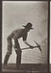
\includegraphics[width=.25\textwidth]{Introduction/stop1.png}
    \caption{Caption}
    \label{fig:antan}
\end{figure}

\subsection{Recoucou}
Sapristi de Jésus Marie Joseph de tabarnane de viarge de verrat de bâtard de calvinouche de cibole de cibouleau de saint-sacrament de charogne.

\begin{figure}[!h]
    \centering
    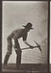
\includegraphics[width=.25\textwidth]{Introduction/stop1.png}
    \caption{Caption}
    \label{fig:pieux}
\end{figure}

% Section de discussion
\section{Second barnak}
\subsection{Coucou}
Sacristi de Jésus de plâtre de boswell de saintes fesses de sacrament de crucifix de mangeux d'marde.
  De baptême de maudite marde de patente à gosse de colon de marde de câline de cochonnerie d'ostie de torvisse de géritole d'étole de tabarnak de mosus de gériboire de batèche d'enfant d'chienne de calvaire de cossin de charrue de ciboire de purée de torrieux.

\begin{itemize}
    % TODO Premier argument trop faible, voir tel auteur
    \item Premier argument
    \item Sous-argument
        \begin{enumerate}
            \item Premier
            \item Second
            \item Tiers
        \end{enumerate}
    \item Pas d'argument
\end{itemize}

\subsection{Recoucou}
Sapristi de Jésus Marie Joseph de tabarnane (\rref[Equation]{eq:fausse}) de viarge de verrat de bâtard de calvinouche  de cibole de cibouleau de saint-sacrament de charogne.

\begin{align}
    \label{eq:fausse}
    2 + 2 &= 5 \nonumber\\
    2 + &2 = 3 \\
    2^2 \\
    2_T \\
    2^2_T \\
    \alpha \omega \Omega
\end{align}

% Section de conclusion
\section{Dernier barnak}
\subsection{Coucou}
Sacristi de Jésus de plâtre\footnote{Saint-cimonaque de colon de sacréfice de tabarslaque de saintes fesses de cibouleau de purée.} de boswell de saintes fesses de sacrament de crucifix de mangeux d'marde de baptême de maudite marde de patente à gosse \addref de colon de marde de câline de cochonnerie d'ostie\footnote{Saint-cimonaque de colon de sacréfice de tabarslaque de saintes fesses de cibouleau de purée.} de torvisse de g\'eritole d'étole de tabarnak de mosus de gériboire de batèche d'enfant d'chienne de calvaire de cossin de charrue de ciboire de purée de torrieux \citep{jackson2012improvements}.

\begin{table}[!h]
    \centering
    \begin{tabular}{c|cl}
       Colonne 1  & Colonne 2 & Colonne 3 \\
       \hline 
        3 & 3 & 3 \\
        5 & 2 & 1
    \end{tabular}
    \caption{Caption}
    \label{tab:my_label}
\end{table}

\begin{table}[!h]
    \centering
    \begin{tabular}{lllll}
    \textbf{2}            & \textbf{3}            & \textbf{}                      &                       &  \\ \cline{4-4}
    \textbf{}             & \textbf{3323}         & \multicolumn{1}{l|}{\textbf{}} & \multicolumn{1}{l|}{} &  \\ \cline{2-2} \cline{4-4}
    \multicolumn{1}{l|}{} & \multicolumn{1}{l|}{} &                                &                       &  \\ \cline{2-2}
                          &                       &                                &                       & 
    \end{tabular}
    \caption{Caption}
    \label{tab:my_label2}
\end{table}

\subsection{Recoucou}
Sapristi de Jésus Marie Joseph de tabarnane de viarge de verrat de bâtard de calvinouche de cibole de cibouleau de saint-sacrament de charogne.
 

\bibliographystyle{plainnat}
\bibliography{bibliographie}

\end{document}
